\documentclass[11pt,a4paper]{article}

% ── packages ──
\usepackage[utf8]{inputenc}
\usepackage[T1]{fontenc}
\usepackage{amsmath,amssymb,amsthm}
\usepackage{algorithm}
\usepackage{algpseudocode}
\usepackage{listings}
\usepackage{xcolor}
\usepackage{geometry}
\usepackage{hyperref}
\usepackage{graphicx}
\usepackage{booktabs}
\usepackage{tikz}
\usetikzlibrary{trees,positioning,arrows.meta}

\geometry{margin=2.4cm}

% ── code listing style ──
\definecolor{codebg}{rgb}{0.96,0.96,0.96}
\definecolor{codegreen}{rgb}{0.0,0.45,0.0}
\definecolor{codegray}{rgb}{0.5,0.5,0.5}
\definecolor{codepurple}{rgb}{0.45,0.0,0.45}
\definecolor{codeblue}{rgb}{0.0,0.0,0.65}

\lstdefinestyle{pythonstyle}{
    backgroundcolor=\color{codebg},
    basicstyle=\ttfamily\small,
    breaklines=true,
    commentstyle=\color{codegreen}\itshape,
    keywordstyle=\color{codeblue}\bfseries,
    stringstyle=\color{codepurple},
    numberstyle=\tiny\color{codegray},
    numbers=left,
    numbersep=6pt,
    frame=single,
    rulecolor=\color{codegray},
    tabsize=4,
    language=Python,
    showstringspaces=false,
    morekeywords={self,None,True,False,np,float64,int8,int32},
    literate={-}{-}1,
    xleftmargin=1.5em,
    framexleftmargin=1.5em,
}
\lstset{style=pythonstyle}

% ── theorem environments ──
\newtheorem{definition}{Definition}[section]
\newtheorem{remark}{Remark}[section]
\newtheorem{example}{Example}[section]

% ── custom commands ──
\newcommand{\logsumexp}{\operatorname{logaddexp}}
\newcommand{\circconv}{\circledast}
\newcommand{\normprod}{\odot}
\DeclareMathOperator*{\argmax}{arg\,max}

% ══════════════════════════════════════════════════════════════════════
\title{%
    \textbf{The Computational Graph SC Decoder\\
    for Two-User MAC Polar Codes}\\[0.8em]
    \large A Line-by-Line Implementation Guide\\
    Based on Ren, Nasser \& Bhatt (2025)
}
\author{Code Reference: \texttt{polar/decoder.py}, Part B}
\date{}

\begin{document}
\maketitle
\tableofcontents
\newpage

% ══════════════════════════════════════════════════════════════════════
\section{Introduction and Motivation}
% ══════════════════════════════════════════════════════════════════════

Consider a two-user binary-input multiple access channel (MAC) where User~1 sends $x^N$ and User~2 sends $y^N$. The receiver observes $z^N$ and must decode both messages.

In the standard successive cancellation (SC) decoder for MAC polar codes, the \textbf{decoding order} is specified by a \emph{path vector} $\mathbf{b}^{2N} \in \{0,1\}^{2N}$. At each of the $2N$ steps, $b_k = 0$ means ``decode the next U~bit'' and $b_k = 1$ means ``decode the next V~bit.''

For \textbf{extreme paths} (all U bits first, then all V bits, or vice versa), a standard LLR-based Arikan SC decoder works efficiently in $O(N \log N)$ time, because one user's codeword is either fully unknown (marginalised) or fully known (conditioned upon).

For \textbf{interleaved paths} such as $\mathbf{b} = 0^{p_i}\, 1^N\, 0^{N - p_i}$ with $0 < p_i < N$, U and V decisions are intermixed. The LLR-based approach breaks down because, at any given step, some bits of the other user are known while others are not. A na\"ive recursive decoder costs $O(N^2)$.

The \textbf{computational graph approach} of Ren, Nasser \& Bhatt (2025) solves this by maintaining $2 \times 2$ log-probability tensors on each edge of a binary tree. It achieves $O(N \log N)$ complexity for \emph{all} monotone chain paths, not just extreme ones.

This document walks through the complete implementation in \texttt{polar/decoder.py}, explaining every function, class, and data structure from first principles to working code.

\subsection{Reading Guide}

\begin{itemize}
    \item \textbf{Section~\ref{sec:background}}: Polar encoding, MAC channels, and the BE-MAC model.
    \item \textbf{Section~\ref{sec:leafprob}}: Building the leaf log-probability array from channel observations.
    \item \textbf{Section~\ref{sec:tensor_ops}}: The two core tensor operations (circular convolution and normalised product).
    \item \textbf{Section~\ref{sec:compgraph}}: The \texttt{\_CompGraph} class --- tree structure, edge data, navigation.
    \item \textbf{Section~\ref{sec:decoder_loop}}: The main SC decoder loop (\texttt{\_decode\_general\_tensor}).
    \item \textbf{Section~\ref{sec:dispatch}}: The public API and auto-dispatch logic.
    \item \textbf{Section~\ref{sec:batch}}: Batch-vectorised decoding for Monte Carlo simulation.
    \item \textbf{Section~\ref{sec:scl}}: Extension to SCL (list) decoding.
    \item \textbf{Section~\ref{sec:usage}}: Complete usage example from encoding to BLER evaluation.
\end{itemize}


% ══════════════════════════════════════════════════════════════════════
\section{Background: Polar Codes on the MAC}
\label{sec:background}
% ══════════════════════════════════════════════════════════════════════

\subsection{Polar Encoding}

The polar code generator matrix is $G_N = B_N \cdot F^{\otimes n}$ where $N = 2^n$,
$F = \begin{psmallmatrix} 1 & 0 \\ 1 & 1 \end{psmallmatrix}$ is the Arikan kernel, and $B_N$ is the bit-reversal permutation matrix.

The encoder applies:
\begin{enumerate}
    \item \textbf{Bit-reversal permutation}: rearrange the input indices according to bit-reversed order.
    \item \textbf{Butterfly stages}: $n = \log_2 N$ stages of XOR operations with doubling step sizes.
\end{enumerate}

\begin{lstlisting}[caption={Polar encoder (\texttt{encoder.py})},label=lst:encoder]
def polar_encode(u) -> list:
    N = len(u)
    n = N.bit_length() - 1
    br = _get_br(n)
    x = np.array(u, dtype=np.int32)[br].copy()  # bit-reversal
    step = 1
    while step < N:
        x_r = x.reshape(-1, 2 * step)
        x_r[:, :step] ^= x_r[:, step:]   # XOR butterfly
        step *= 2
    return x.tolist()
\end{lstlisting}

The reshape trick on line~8 views the flat array as blocks of size $2 \cdot \texttt{step}$, then XORs the left half with the right half. After $\log_2 N$ stages, the output $x^N$ is the polar-encoded codeword.

\subsection{The BE-MAC Channel}

The Binary Erasure MAC (BE-MAC) is defined by $Z = X + Y$ where $X, Y \in \{0, 1\}$ and $Z \in \{0, 1, 2\}$. It is deterministic (no noise):
\[
W(z \mid x, y) = \begin{cases} 1 & \text{if } z = x + y, \\ 0 & \text{otherwise.} \end{cases}
\]

The capacity region is:
\[
R_u \leq I(Z; X) = 0.5, \quad R_v \leq I(Z; Y \mid X) = 1.0, \quad R_u + R_v \leq 1.5.
\]

\subsection{Monotone Chain Paths}

A \emph{monotone chain path} has the form $\mathbf{b} = 0^{p_i}\, 1^N\, 0^{N - p_i}$ for some $p_i \in \{0, 1, \ldots, N\}$. The parameter $p_i$ is called the \textbf{path index}:
\begin{itemize}
    \item $p_i = N$: decode all U first, then all V (``U-first,'' extreme path, Code Class~C).
    \item $p_i = 0$: decode all V first, then all U (``V-first,'' extreme path).
    \item $0 < p_i < N$: interleaved decoding (Code Classes A and B).
\end{itemize}

The path is constructed by:
\begin{lstlisting}[caption={Path construction (\texttt{design.py})}]
def make_path(N: int, path_i: int) -> list:
    return [0] * path_i + [1] * N + [0] * (N - path_i)
\end{lstlisting}

\subsection{Code Design}

Given a code class with target rates $(R_u^{\mathrm{dir}}, R_v^{\mathrm{dir}})$, and a rate-scaling parameter $\rho \in (0, 1]$, the number of information bits is:
\[
k_u = \lfloor \rho \cdot R_u^{\mathrm{dir}} \cdot N \rceil, \qquad
k_v = \lfloor \rho \cdot R_v^{\mathrm{dir}} \cdot N \rceil.
\]

The \texttt{design\_bemac(n, ku, kv)} function uses Bhattacharyya parameter analysis to select the $k_u$ most reliable U sub-channels (information set $\mathcal{A}_u$) and the $k_v$ most reliable V sub-channels ($\mathcal{A}_v$). All other positions are \textbf{frozen} to zero.


% ══════════════════════════════════════════════════════════════════════
\section{Leaf Log-Probabilities}
\label{sec:leafprob}
% ══════════════════════════════════════════════════════════════════════

The computational graph decoder operates on $2 \times 2$ log-probability tensors. The \textbf{leaf tensors} are computed directly from the channel observations $z^N$ and the channel transition probabilities.

\begin{definition}[Leaf log-probability]
For time index $t \in \{0, \ldots, N-1\}$, the leaf tensor is the $2 \times 2$ matrix:
\[
\log W_t[x, y] = \log W(z_t \mid x, y), \qquad x, y \in \{0, 1\}.
\]
The full leaf array has shape $(N, 2, 2)$.
\end{definition}

\begin{lstlisting}[caption={Building leaf log-probabilities (\texttt{build\_log\_W\_leaf})}]
def build_log_W_leaf(z, channel) -> np.ndarray:
    N = len(z)

    if channel.name == "be_mac":
        xy_sum = np.array([[0, 1], [1, 2]], dtype=np.int32)
        z_arr = np.asarray(z, dtype=np.int32)
        match = z_arr[:, None, None] == xy_sum[None, :, :]
        log_W = np.where(match, 0.0, -np.inf)

    return log_W
\end{lstlisting}

\paragraph{How it works.} The constant array \texttt{xy\_sum[x, y] = x + y} has shape $(2, 2)$. The comparison \texttt{z\_arr[:, None, None] == xy\_sum[None, :, :]} broadcasts to shape $(N, 2, 2)$ and produces \texttt{True} exactly where $z_t = x + y$. The \texttt{np.where} maps \texttt{True} $\to 0.0$ (i.e.\ $\log 1 = 0$) and \texttt{False} $\to -\infty$ (i.e.\ $\log 0$).

\begin{example}
For $N = 4$ and $z = [0, 1, 2, 1]$:
\[
\log W_0 = \begin{pmatrix} 0 & -\infty \\ -\infty & -\infty \end{pmatrix}, \quad
\log W_1 = \begin{pmatrix} -\infty & 0 \\ 0 & -\infty \end{pmatrix}, \quad
\log W_2 = \begin{pmatrix} -\infty & -\infty \\ -\infty & 0 \end{pmatrix}, \quad
\log W_3 = \begin{pmatrix} -\infty & 0 \\ 0 & -\infty \end{pmatrix}.
\]
The entry $\log W_0[0,0] = 0$ because $z_0 = 0 = 0 + 0$ is consistent with $(x,y) = (0,0)$.
\end{example}


% ══════════════════════════════════════════════════════════════════════
\section{Core Tensor Operations}
\label{sec:tensor_ops}
% ══════════════════════════════════════════════════════════════════════

The computational graph relies on two operations on $2 \times 2$ log-probability tensors: \textbf{circular convolution} $\circconv$ and \textbf{normalised product} $\normprod$.

\subsection{Circular Convolution ($\circconv$)}
\label{subsec:circ_conv}

\begin{definition}[Circular convolution, Eq.~13--14 of Ren et al.]
For two $2 \times 2$ log-probability tensors $A$ and $B$:
\[
(A \circconv B)[a, b] = \log \sum_{a', b' \in \{0,1\}} \exp\!\big( A[a \oplus a',\, b \oplus b'] + B[a', b'] \big)
\]
where $\oplus$ denotes XOR (addition modulo 2).
\end{definition}

This is a convolution over the group $\mathbb{Z}_2 \times \mathbb{Z}_2$. Each output entry is a log-sum-exp of four terms. For the $(0,0)$ entry:
\[
(A \circconv B)[0,0] = \logsumexp\big(A_{00} + B_{00},\; A_{01} + B_{01},\; A_{10} + B_{10},\; A_{11} + B_{11}\big).
\]

\paragraph{Physical meaning.} Circular convolution \emph{marginalises out an unknown variable}. If $A$ represents $\log P(z_{\text{left}} \mid x, y)$ and $B$ represents $\log P(z_{\text{right}} \mid x, y)$, then $A \circconv B$ represents the joint probability when the left and right sub-blocks share independent encoding (the ``bad'' channel split $W^-$ in Arikan's terminology).

\begin{lstlisting}[caption={Circular convolution (\texttt{\_circ\_conv\_batch})},label=lst:circ_conv]
def _circ_conv_batch(A, B):
    """
    Vectorized circular convolution of (L, 2, 2)
    log-prob tensor arrays.
    """
    A00 = A[:, 0, 0]; A01 = A[:, 0, 1]
    A10 = A[:, 1, 0]; A11 = A[:, 1, 1]
    B00 = B[:, 0, 0]; B01 = B[:, 0, 1]
    B10 = B[:, 1, 0]; B11 = B[:, 1, 1]

    out = np.empty_like(A)
    out[:, 0, 0] = np.logaddexp(
        np.logaddexp(A00 + B00, A01 + B01),
        np.logaddexp(A10 + B10, A11 + B11))
    out[:, 0, 1] = np.logaddexp(
        np.logaddexp(A01 + B00, A00 + B01),
        np.logaddexp(A11 + B10, A10 + B11))
    out[:, 1, 0] = np.logaddexp(
        np.logaddexp(A10 + B00, A11 + B01),
        np.logaddexp(A00 + B10, A01 + B11))
    out[:, 1, 1] = np.logaddexp(
        np.logaddexp(A11 + B00, A10 + B01),
        np.logaddexp(A01 + B10, A00 + B11))
    return out
\end{lstlisting}

\paragraph{Implementation notes.}
\begin{itemize}
    \item The function is \emph{vectorised}: it operates on arrays of $L$ tensors simultaneously (shape $(L, 2, 2)$). This is critical for the computational graph where each edge stores $N / 2^j$ tensors at level~$j$.
    \item \texttt{np.logaddexp(a, b)} computes $\log(\exp(a) + \exp(b))$ in a numerically stable way, correctly handling $-\infty$ inputs.
    \item The nested \texttt{logaddexp} calls implement a binary tree reduction: $\logsumexp(a, b, c, d) = \logsumexp(\logsumexp(a, b), \logsumexp(c, d))$.
    \item Each output entry involves exactly 4 additions and 3 \texttt{logaddexp} calls.
\end{itemize}

\subsection{Normalised Product ($\normprod$)}
\label{subsec:norm_prod}

\begin{definition}[Normalised product]
For two $2 \times 2$ log-probability tensors $A$ and $B$:
\[
(A \normprod B)[a, b] = A[a, b] + B[a, b] - \log \sum_{a', b'} \exp\!\big(A[a', b'] + B[a', b']\big).
\]
\end{definition}

This is elementwise multiplication in probability domain, followed by normalisation. In log domain, it becomes addition followed by subtraction of the log-partition function.

\paragraph{Physical meaning.} The normalised product \emph{combines two independent pieces of evidence} about the same variable. If $A$ is a top-down message and $B$ is a bottom-up message, $A \normprod B$ gives the posterior.

\begin{lstlisting}[caption={Normalised product (\texttt{\_norm\_prod\_batch} and \texttt{\_norm\_prod\_single})}]
def _norm_prod_batch(A, B):
    """Vectorized normalised product of (L, 2, 2) arrays."""
    raw = A + B
    total = np.logaddexp(
        np.logaddexp(raw[:, 0, 0], raw[:, 0, 1]),
        np.logaddexp(raw[:, 1, 0], raw[:, 1, 1])
    )
    finite = np.isfinite(total)
    result = raw.copy()
    result[finite] -= total[finite, None, None]
    return result


def _norm_prod_single(A, B):
    """Normalised product for single 2x2 tensors."""
    raw = A + B
    total = np.logaddexp(
        np.logaddexp(raw[0, 0], raw[0, 1]),
        np.logaddexp(raw[1, 0], raw[1, 1])
    )
    if np.isfinite(total):
        return raw - total
    return raw.copy()
\end{lstlisting}

\paragraph{Implementation notes.}
\begin{itemize}
    \item \texttt{raw = A + B} computes the unnormalised log-product elementwise.
    \item \texttt{total} is the log-partition function (log of the sum of all four entries' exponentials).
    \item The \texttt{finite} guard handles the case where all four entries are $-\infty$ (total would be $-\infty$, and subtraction would produce \texttt{NaN}). In that case, the result is left as all $-\infty$.
    \item The \texttt{\_single} variant operates on a single $(2, 2)$ tensor, used at leaf nodes during decoding.
\end{itemize}


% ══════════════════════════════════════════════════════════════════════
\section{The Computational Graph (\texttt{\_CompGraph})}
\label{sec:compgraph}
% ══════════════════════════════════════════════════════════════════════

The \texttt{\_CompGraph} class maintains the state of the SC decoder as a binary tree of $2 \times 2$ log-probability tensors. It implements Algorithms~3--6 of Ren et al.\ (2025).

\subsection{Tree Indexing}

\begin{definition}[Edge and vertex indexing]
For a code of length $N = 2^n$:
\begin{itemize}
    \item \textbf{Edges} are numbered $1, 2, \ldots, 2N - 1$.
    \item Edge~1 is the \textbf{root} (channel posterior).
    \item Edges $N, N+1, \ldots, 2N-1$ are the \textbf{leaves}.
    \item \textbf{Vertices} are numbered $1, 2, \ldots, N-1$.
    \item Vertex $\beta$ has:
    \begin{itemize}
        \item parent edge $\beta$,
        \item left child edge $2\beta$,
        \item right child edge $2\beta + 1$.
    \end{itemize}
    \item Edge $\beta$ at level $j = \lfloor \log_2 \beta \rfloor$ stores $N / 2^j$ tensors of shape $(2, 2)$.
\end{itemize}
\end{definition}

\begin{figure}[h]
\centering
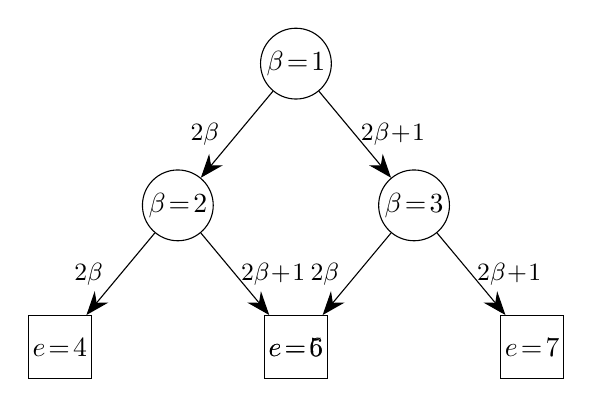
\begin{tikzpicture}[
    level distance=1.8cm,
    sibling distance=3cm,
    edge from parent/.style={draw,-{Stealth[length=3mm]}},
    every node/.style={draw, circle, minimum size=8mm, inner sep=1pt}
]
\node {$\beta\!=\!1$}
    child { node {$\beta\!=\!2$}
        child { node[rectangle] {$e\!=\!4$} edge from parent node[left,draw=none] {\small$2\beta$} }
        child { node[rectangle] {$e\!=\!5$} edge from parent node[right,draw=none] {\small$2\beta\!+\!1$} }
        edge from parent node[left,draw=none] {\small$2\beta$}
    }
    child { node {$\beta\!=\!3$}
        child { node[rectangle] {$e\!=\!6$} edge from parent node[left,draw=none] {\small$2\beta$} }
        child { node[rectangle] {$e\!=\!7$} edge from parent node[right,draw=none] {\small$2\beta\!+\!1$} }
        edge from parent node[right,draw=none] {\small$2\beta\!+\!1$}
    };
\end{tikzpicture}
\caption{Binary tree for $N = 4$ ($n = 2$). Circles are vertices (1--3), rectangles are leaf edges (4--7). Edge~1 (root) connects to vertex~1 from above (not shown).}
\label{fig:tree}
\end{figure}

\begin{example}[Edge sizes for $N = 8$]
\begin{center}
\begin{tabular}{cccc}
\toprule
Edge $\beta$ & Level $j$ & Size $N/2^j$ & Data shape \\
\midrule
1 & 0 & 8 & $(8, 2, 2)$ \\
2, 3 & 1 & 4 & $(4, 2, 2)$ \\
4, 5, 6, 7 & 2 & 2 & $(2, 2, 2)$ \\
8, 9, \ldots, 15 & 3 & 1 & $(1, 2, 2)$ \\
\bottomrule
\end{tabular}
\end{center}
Total tensors stored: $8 + 2 \times 4 + 4 \times 2 + 8 \times 1 = 8 + 8 + 8 + 8 = 32 = (n+1) \cdot N$.
\end{example}

\subsection{Initialisation}

\begin{lstlisting}[caption={Graph initialisation (\texttt{\_CompGraph.\_\_init\_\_})}]
class _CompGraph:
    def __init__(self, n, log_W_leaf):
        self.n = n
        self.N = 1 << n
        N = self.N

        self.edge_data = [None] * (2 * N)

        from .encoder import bit_reversal_perm
        br = bit_reversal_perm(n)
        root = log_W_leaf[br].copy()
        totals = np.logaddexp(
            np.logaddexp(root[:, 0, 0], root[:, 0, 1]),
            np.logaddexp(root[:, 1, 0], root[:, 1, 1])
        )
        finite = np.isfinite(totals)
        root[finite] -= totals[finite, None, None]
        self.edge_data[1] = root

        for beta in range(2, 2 * N):
            level = beta.bit_length() - 1
            size = N >> level
            self.edge_data[beta] = np.full((size, 2, 2),
                                           _LOG_QUARTER,
                                           dtype=np.float64)

        self.dec_head = 1
\end{lstlisting}

\paragraph{Step-by-step explanation.}
\begin{enumerate}
    \item \textbf{Line 7}: Allocate a Python list of length $2N$ for edge data. Index~0 is unused; edges are indexed 1 to $2N - 1$.

    \item \textbf{Lines 9--11}: The leaf log-probabilities are reordered according to the \textbf{bit-reversal permutation}. This is essential because the encoder applies bit-reversal before the butterfly, and the tree's left/right splitting (pairing position $i$ with position $i + \ell$) must match the $F^{\otimes n}$ decomposition.

    \item \textbf{Lines 12--18}: Each $2 \times 2$ tensor in the root is \textbf{normalised} by subtracting the log-partition function. This ensures $\sum_{x,y} \exp(\text{root}[t, x, y]) = 1$ for each~$t$. The \texttt{finite} guard prevents subtracting $-\infty$ from $-\infty$.

    \item \textbf{Line 19}: Store the normalised root at edge~1. Its shape is $(N, 2, 2)$.

    \item \textbf{Lines 21--25}: All non-root edges are initialised to the \textbf{uniform distribution}: $\log(1/4)$ in all four entries. This represents ``no information'' --- the prior for undecided leaves. The size of edge $\beta$ is $N / 2^{\mathrm{level}}$ where $\mathrm{level} = \lfloor \log_2 \beta \rfloor$.

    \item \textbf{Line 27}: The \texttt{dec\_head} pointer tracks which vertex the decoder is currently ``sitting at.'' It starts at vertex~1 (the root).
\end{enumerate}

\begin{remark}[Why bit-reversal?]
The tree's internal pairing at each level matches the interleaved structure of $F^{\otimes n}$. Position $i$ is paired with position $i + \ell$ (where $\ell$ is the half-size at that level). Since the encoder applies $B_N$ first, the root entries must also be bit-reversed so the tree decomposition corresponds to the actual code structure.
\end{remark}

\subsection{The Three Core Operations}
\label{subsec:calc_ops}

The computational graph has three operations that propagate information through the tree.

\subsubsection{calcLeft (Eq.~13): Top-Down to Left Child}

\begin{lstlisting}[caption={calcLeft operation}]
def calc_left(self, beta):
    parent = self.edge_data[beta]
    right = self.edge_data[2 * beta + 1]
    l = right.shape[0]
    temp = _norm_prod_batch(parent[l:], right)
    self.edge_data[2 * beta] = _circ_conv_batch(
        parent[:l], temp)
\end{lstlisting}

\paragraph{Explanation.} At vertex $\beta$, the parent edge has $2\ell$ tensors (where $\ell$ is the child size). We split the parent into two halves: \texttt{parent[:l]} and \texttt{parent[l:]}.

\begin{enumerate}
    \item \textbf{Combine evidence}: \texttt{temp = \_norm\_prod\_batch(parent[l:], right)} merges the bottom half of the parent with the right child's bottom-up information.
    \item \textbf{Marginalise}: \texttt{\_circ\_conv\_batch(parent[:l], temp)} performs the circular convolution (marginalisation over the unknown bit), producing the left child's top-down message.
\end{enumerate}

Intuitively: to compute the message going \emph{down} to the left child, we need to incorporate what we know from the right subtree (bottom-up) and the channel (top-down from parent).

\subsubsection{calcRight (Eq.~14): Top-Down to Right Child}

\begin{lstlisting}[caption={calcRight operation}]
def calc_right(self, beta):
    parent = self.edge_data[beta]
    left = self.edge_data[2 * beta]
    l = left.shape[0]
    temp = _circ_conv_batch(left, parent[:l])
    self.edge_data[2 * beta + 1] = _norm_prod_batch(
        parent[l:], temp)
\end{lstlisting}

\paragraph{Explanation.} This is the dual of calcLeft. The order of operations is reversed: first circular convolution (with the left child), then normalised product (with the parent's bottom half).

Intuitively: to send a message down to the right child, we first incorporate the left child's information (bottom-up) via convolution, then combine with the parent's top-down information.

\subsubsection{calcParent (Eq.~15): Bottom-Up to Parent}

\begin{lstlisting}[caption={calcParent operation}]
def calc_parent(self, beta):
    left = self.edge_data[2 * beta]
    right = self.edge_data[2 * beta + 1]
    l = left.shape[0]
    parent = np.empty((2 * l, 2, 2), dtype=np.float64)
    parent[:l] = _circ_conv_batch(left, right)
    parent[l:] = right
    self.edge_data[beta] = parent
\end{lstlisting}

\paragraph{Explanation.} When stepping \emph{up} from a child to its parent:
\begin{enumerate}
    \item The top half of the parent is the circular convolution of left and right children.
    \item The bottom half is simply a copy of the right child.
\end{enumerate}

This corresponds to the factorisation of the polar code: the parent's distribution factors into a ``bad'' channel (convolution of children) and a ``good'' channel (right child, conditioned on the left).

\begin{remark}[Key subtlety: calcParent direction]
When navigating \emph{up} from the current vertex to its parent, \texttt{calcParent} is called on the \textbf{current vertex} (not the target parent). This converts the current vertex's edge from a ``getAsChild'' representation to a ``getAsParent'' representation. The root edge (edge~1) is never overwritten by calcParent.
\end{remark}

\subsection{Navigation: step\_to, \_step\_one, \_get\_path}
\label{subsec:navigation}

The decoder needs to move its ``decode head'' between vertices to visit each leaf. The navigation system implements Algorithms~5 and~6 of Ren et al.

\begin{lstlisting}[caption={Navigation (\texttt{step\_to}, \texttt{\_step\_one}, \texttt{\_get\_path})}]
def step_to(self, target):
    current = self.dec_head
    if current == target:
        return
    path = self._get_path(current, target)
    for beta in path:
        self._step_one(beta)
    self.dec_head = target

def _step_one(self, beta):
    current = self.dec_head
    if current == beta >> 1:      # going DOWN
        if beta & 1 == 0:
            self.calc_left(current)
        else:
            self.calc_right(current)
        self.dec_head = beta
    elif beta == current >> 1:    # going UP
        self.calc_parent(current)
        self.dec_head = beta

def _get_path(self, current, target):
    if current == target:
        return []
    path_up = []
    path_down = []
    c, t = current, target
    while c != t:
        if c > t:
            c = c >> 1
            path_up.append(c)
        else:
            path_down.append(t)
            t = t >> 1
    path_down.reverse()
    return path_up + path_down
\end{lstlisting}

\paragraph{How \texttt{\_get\_path} works.}
The algorithm finds the \textbf{lowest common ancestor (LCA)} of \texttt{current} and \texttt{target} by alternately dividing the larger index by 2. It collects:
\begin{itemize}
    \item \texttt{path\_up}: vertices to visit going up from \texttt{current} to the LCA.
    \item \texttt{path\_down}: vertices to visit going down from the LCA to \texttt{target}.
\end{itemize}
The result is concatenated: first go up, then go down.

\paragraph{How \texttt{\_step\_one} works.}
Each step is either:
\begin{itemize}
    \item \textbf{Going down} ($\texttt{current} = \beta \gg 1$): current vertex is the parent of $\beta$. Call calcLeft or calcRight depending on whether $\beta$ is a left child (even) or right child (odd).
    \item \textbf{Going up} ($\beta = \texttt{current} \gg 1$): $\beta$ is the parent of current. Call calcParent on the current vertex (not $\beta$!).
\end{itemize}

\begin{example}[Navigation for $N = 8$]
Suppose the decode head is at vertex~5 and we need to reach vertex~2. The path is:
\begin{enumerate}
    \item From 5: $5 > 2$, so go up. $5 \gg 1 = 2$, so path\_up = [2]. Now $c = 2 = t$.
    \item The LCA is vertex~2. Path = [2]. One step: calcParent at current vertex~5, move to vertex~2.
\end{enumerate}
\end{example}


% ══════════════════════════════════════════════════════════════════════
\section{The Main Decoder Loop}
\label{sec:decoder_loop}
% ══════════════════════════════════════════════════════════════════════

The function \texttt{\_decode\_general\_tensor} implements Algorithm~4 of Ren et al.\ (2025). It performs $2N$ steps, one for each element of the path vector~$\mathbf{b}$.

\begin{lstlisting}[caption={Main decoder loop (\texttt{\_decode\_general\_tensor})},label=lst:main_loop]
def _decode_general_tensor(N, log_W, b, frozen_u, frozen_v):
    n = N.bit_length() - 1
    graph = _CompGraph(n, log_W)

    u_hat = {}   # 1-indexed position -> decided value
    v_hat = {}
    i_u = 0      # U-bit counter
    i_v = 0      # V-bit counter

    for step in range(2 * N):
        gamma = b[step]   # 0 = U step, 1 = V step

        if gamma == 0:
            i_u += 1
            i_t = i_u
            frozen_dict = frozen_u
        else:
            i_v += 1
            i_t = i_v
            frozen_dict = frozen_v

        leaf_edge = i_t + N - 1
        target_vertex = leaf_edge >> 1

        # --- Navigate to leaf's parent ---
        graph.step_to(target_vertex)

        # --- Save bottom-up data ---
        temp = graph.edge_data[leaf_edge][0].copy()

        # --- Compute top-down message ---
        if leaf_edge & 1 == 0:
            graph.calc_left(target_vertex)
        else:
            graph.calc_right(target_vertex)

        top_down = graph.edge_data[leaf_edge][0]

        # --- Combine and decide ---
        combined = _norm_prod_single(top_down, temp)

        if i_t in frozen_dict:
            bit = frozen_dict[i_t]
        else:
            if gamma == 0:   # U decision: marginalise over V
                p0 = np.logaddexp(combined[0, 0],
                                  combined[0, 1])
                p1 = np.logaddexp(combined[1, 0],
                                  combined[1, 1])
                bit = 1 if p1 > p0 else 0
            else:            # V decision: marginalise over U
                p0 = np.logaddexp(combined[0, 0],
                                  combined[1, 0])
                p1 = np.logaddexp(combined[0, 1],
                                  combined[1, 1])
                bit = 1 if p1 > p0 else 0

        # --- Record decision ---
        if gamma == 0:
            u_hat[i_t] = bit
        else:
            v_hat[i_t] = bit

        # --- Update leaf (partially deterministic) ---
        new_leaf = np.full((2, 2), _NEG_INF, dtype=np.float64)
        u_val = u_hat.get(i_t)
        v_val = v_hat.get(i_t)

        if u_val is not None and v_val is not None:
            new_leaf[u_val, v_val] = 0.0
        elif u_val is not None:
            new_leaf[u_val, 0] = _LOG_HALF
            new_leaf[u_val, 1] = _LOG_HALF
        elif v_val is not None:
            new_leaf[0, v_val] = _LOG_HALF
            new_leaf[1, v_val] = _LOG_HALF
        else:
            new_leaf[:, :] = _LOG_QUARTER

        graph.edge_data[leaf_edge][0] = new_leaf

    u_dec = [u_hat.get(k, 0) for k in range(1, N + 1)]
    v_dec = [v_hat.get(k, 0) for k in range(1, N + 1)]
    return u_dec, v_dec
\end{lstlisting}

\subsection{Detailed Walkthrough}

We now explain each phase of one iteration of the main loop.

\subsubsection{Phase 1: Identify the Current Step (Lines 11--20)}

The path vector $\mathbf{b}$ determines whether this step decodes a U~bit ($\gamma = 0$) or a V~bit ($\gamma = 1$). The counters \texttt{i\_u} and \texttt{i\_v} track how many U and V bits have been decided so far. The variable \texttt{i\_t} is the \textbf{1-indexed position} within the respective user's message.

\subsubsection{Phase 2: Locate the Leaf (Lines 22--23)}

Each leaf position \texttt{i\_t} maps to a leaf edge:
\[
\texttt{leaf\_edge} = i_t + N - 1.
\]
The parent vertex is:
\[
\texttt{target\_vertex} = \lfloor \texttt{leaf\_edge} / 2 \rfloor.
\]

\begin{example}
For $N = 8$ and $i_t = 3$: leaf edge $= 3 + 8 - 1 = 10$, target vertex $= 5$.
\end{example}

\subsubsection{Phase 3: Navigate (Line 26)}

The decoder moves its \texttt{dec\_head} from wherever it is to \texttt{target\_vertex}. This may involve multiple calcLeft/calcRight/calcParent operations along the path.

\subsubsection{Phase 4: Save Bottom-Up Data (Line 29)}

Before computing the top-down message, we \textbf{save} the leaf's current data. This is the bottom-up information from previous decisions (or the uniform prior if this leaf hasn't been visited).

The \texttt{[0]} index selects the single $(2, 2)$ tensor stored at this leaf edge (leaf edges have size~1).

\subsubsection{Phase 5: Compute Top-Down Message (Lines 31--36)}

We call calcLeft or calcRight on the target vertex, which overwrites the leaf edge's data with the \textbf{top-down message} --- the information flowing from the root towards this leaf.

The choice between calcLeft and calcRight depends on whether the leaf edge is a left child (even index) or right child (odd index) of the target vertex.

\subsubsection{Phase 6: Combine and Decide (Lines 38--55)}

The \textbf{combined} posterior is the normalised product of the top-down message and the saved bottom-up data:
\[
\texttt{combined}[x, y] = \texttt{top\_down}[x, y] + \texttt{temp}[x, y] - \text{normalisation}.
\]

For a \textbf{U~decision} (marginalise over~V):
\[
P(u = b) = \sum_{y} \exp(\texttt{combined}[b, y]) = \exp\big(\logsumexp(\texttt{combined}[b, 0], \texttt{combined}[b, 1])\big).
\]
The decoder chooses $\hat{u} = \argmax_b P(u = b)$.

For a \textbf{V~decision} (marginalise over~U):
\[
P(v = b) = \sum_{x} \exp(\texttt{combined}[x, b]).
\]

If the position is \textbf{frozen}, the decoder uses the predetermined frozen value instead.

\subsubsection{Phase 7: Update Leaf Tensor (Lines 62--80)}

After deciding, the leaf tensor is updated to a \textbf{partially deterministic} distribution (Eq.~16 of Ren et al.):

\begin{itemize}
    \item \textbf{Both $u$ and $v$ decided} at this position: delta function at $(\hat{u}, \hat{v})$.
    \[
    \texttt{new\_leaf}[\hat{u}, \hat{v}] = 0, \quad \text{all other entries} = -\infty.
    \]

    \item \textbf{Only $u$ decided}: known $u = \hat{u}$, uniform over $v$.
    \[
    \texttt{new\_leaf}[\hat{u}, 0] = \texttt{new\_leaf}[\hat{u}, 1] = \log(1/2), \quad \text{other row} = -\infty.
    \]

    \item \textbf{Only $v$ decided}: known $v = \hat{v}$, uniform over $u$.
    \[
    \texttt{new\_leaf}[0, \hat{v}] = \texttt{new\_leaf}[1, \hat{v}] = \log(1/2), \quad \text{other column} = -\infty.
    \]

    \item \textbf{Neither decided}: uniform over both.
    \[
    \texttt{new\_leaf}[x, y] = \log(1/4) \quad \forall x, y.
    \]
\end{itemize}

\begin{remark}[Why partially deterministic, not the combined posterior?]
One might think we should store the full combined posterior at the leaf after deciding. This would be \textbf{incorrect}: it would double-count the channel information when the leaf is revisited later (during the second user's decision at the same position). Instead, the partially deterministic tensor encodes \emph{only} the decision, with uniform distribution over the undecided dimension.
\end{remark}

\subsubsection{Phase 8: Collect Results (Lines 82--84)}

After all $2N$ steps, the decisions are collected into lists. Positions not in \texttt{u\_hat} or \texttt{v\_hat} default to~0 (they are frozen positions that were never explicitly visited, which means they must have value~0).


% ══════════════════════════════════════════════════════════════════════
\section{Public API and Auto-Dispatch}
\label{sec:dispatch}
% ══════════════════════════════════════════════════════════════════════

The public function \texttt{decode\_single} auto-dispatches between the LLR-based decoder (for extreme paths) and the tensor-based decoder (for all other paths):

\begin{lstlisting}[caption={Public API (\texttt{decode\_single})}]
def decode_single(N, z, b, frozen_u, frozen_v, channel,
                  log_domain=True):
    path_i = _detect_path_i(N, b)
    log_W = build_log_W_leaf(z, channel)

    if path_i == 0 or path_i == N:
        return _decode_extreme_llr(N, log_W, path_i,
                                   frozen_u, frozen_v)
    else:
        return _decode_general_tensor(N, log_W, b,
                                      frozen_u, frozen_v)
\end{lstlisting}

The function \texttt{\_detect\_path\_i} examines the path vector to determine if it has the monotone chain structure $0^{p_i} 1^N 0^{N - p_i}$. If $p_i = 0$ or $p_i = N$, the LLR-based decoder is used (approximately $2\times$ faster). Otherwise, the tensor-based computational graph decoder handles the interleaved path.


% ══════════════════════════════════════════════════════════════════════
\section{Batch-Vectorised Decoding}
\label{sec:batch}
% ══════════════════════════════════════════════════════════════════════

For Monte Carlo simulation, we need to decode thousands of codewords. Processing them one-at-a-time is slow due to Python loop overhead. The batch decoder processes all codewords \textbf{simultaneously} by adding a \emph{batch dimension} to every array.

\subsection{Key Idea}

The SC decoder has $2N$ inherently sequential steps (each decision depends on previous ones). However, within each step, the tensor operations can be vectorised across codewords. The Python loop stays the same; only the NumPy arrays grow from $(L, 2, 2)$ to $(\text{batch}, L, 2, 2)$.

\subsection{Batched Computational Graph}

\begin{lstlisting}[caption={Batched computational graph (\texttt{\_CompGraphBatched})}]
class _CompGraphBatched:
    def __init__(self, n, log_W_batch):
        # log_W_batch: (batch, N, 2, 2)
        self.batch = log_W_batch.shape[0]
        ...
        # edge_data[beta]: shape (batch, size, 2, 2)
        root = log_W_batch[:, br].copy()  # (batch, N, 2, 2)
        self.edge_data[1] = root
        ...

    def calc_left(self, beta):
        parent = self.edge_data[beta]    # (batch, 2l, 2, 2)
        right = self.edge_data[2*beta+1] # (batch, l, 2, 2)
        l = right.shape[1]
        temp = _norm_prod_batched(parent[:, l:], right)
        self.edge_data[2*beta] = _circ_conv_batched(
            parent[:, :l], temp)
\end{lstlisting}

The only changes from the single-codeword version:
\begin{itemize}
    \item All edge data shapes gain a leading batch dimension.
    \item \texttt{\_circ\_conv\_batched(A, B)} reshapes $(B, L, 2, 2)$ to $(B \cdot L, 2, 2)$, calls the existing \texttt{\_circ\_conv\_batch}, and reshapes back.
    \item Navigation logic is identical (it only uses Python integer indices).
\end{itemize}

\subsection{Batched Decision-Making}

In the batched decoder, bit decisions are vectorised:

\begin{lstlisting}[caption={Vectorised bit decisions}]
# Instead of:  bit = 1 if p1 > p0 else 0
# Batched:
bit = (p1 > p0).astype(np.int32)   # shape (batch,)
\end{lstlisting}

Similarly, leaf updates use advanced NumPy indexing:

\begin{lstlisting}[caption={Vectorised leaf update}]
new_leaf = np.full((batch, 2, 2), _NEG_INF)
# Both u and v decided:
new_leaf[np.arange(batch), u_val, v_val] = 0.0
\end{lstlisting}

\subsection{Performance}

The batch decoder achieves $30$--$50\times$ speedup over sequential decoding:

\begin{center}
\begin{tabular}{lccc}
\toprule
& Class A (general) & Class B (general) & Class C (extreme) \\
\midrule
$N = 64$, 200 cw & $36\times$ & $38\times$ & $52\times$ \\
$N = 1024$, 20 cw & $12\times$ & $12\times$ & $10\times$ \\
\bottomrule
\end{tabular}
\end{center}

The speedup decreases at larger $N$ because the per-step NumPy operations become more compute-bound (less overhead-dominated).


% ══════════════════════════════════════════════════════════════════════
\section{Extension to SCL Decoding}
\label{sec:scl}
% ══════════════════════════════════════════════════════════════════════

The SCL (Successive Cancellation List) decoder extends SC by maintaining $L$ candidate paths in parallel. At each information bit, each path forks into two candidates (bit~0 and bit~1), and the worst paths are pruned.

\subsection{Packed Batch Graph (\texttt{\_BatchCompGraph})}

The SCL decoder in \texttt{decoder\_scl.py} uses a \texttt{\_BatchCompGraph} that packs all $L$ paths' edge data into a single contiguous array:

\begin{lstlisting}[caption={SCL packed graph (\texttt{\_BatchCompGraph})}]
class _BatchCompGraph:
    def __init__(self, n, log_W_leaf, max_paths):
        # Packed layout: all edges concatenated
        total = sum(N >> (beta.bit_length()-1)
                    for beta in range(1, 2*N))
        self._data = np.full(
            (max_paths, total, 2, 2),
            _LOG_QUARTER, dtype=np.float64)
        ...

    def _e(self, beta):
        """View of edge beta for all paths."""
        o, s = self._off[beta], self._sz[beta]
        return self._data[:, o:o+s]

    def copy_path(self, dst, src):
        """Copy all edge data: single array op."""
        self._data[dst] = self._data[src]
\end{lstlisting}

\textbf{Key advantage}: path copying (needed during fork-and-prune) is a single array slice assignment, which is very fast.

\subsection{Fork and Prune}

At each information bit $\phi$:
\begin{enumerate}
    \item Each active path $l$ produces two candidates: $(l, \text{bit}=0)$ with metric $\text{PM}[l] + P_0[l]$, and $(l, \text{bit}=1)$ with metric $\text{PM}[l] + P_1[l]$.
    \item All candidates are sorted by metric (descending).
    \item The best $L$ candidates survive; the rest are pruned.
    \item Surviving candidates that need a different slot get their data \emph{copied} from the source path.
\end{enumerate}


% ══════════════════════════════════════════════════════════════════════
\section{Complete Usage Example}
\label{sec:usage}
% ══════════════════════════════════════════════════════════════════════

The following shows the complete pipeline from code design to BLER evaluation.

\begin{lstlisting}[caption={Complete pipeline example}]
import numpy as np
from polar import (polar_encode, build_message, BEMAC,
                   design_bemac, make_path,
                   decode_single, decode_batch)
from polar.encoder import polar_encode_batch, build_message_batch

# --- Setup ---
N = 64; n = 6
channel = BEMAC()

# Code Class B: interleaved path
path_i = round(0.5 * N)   # = 32
b = make_path(N, path_i)  # [0]*32 + [1]*64 + [0]*32

# Rate rho = 0.7
Ru_dir, Rv_dir = 0.625, 0.875
ku = round(0.7 * Ru_dir * N)  # = 28
kv = round(0.7 * Rv_dir * N)  # = 39
Au, Av, frozen_u, frozen_v, _, _ = design_bemac(n, ku, kv)

# --- Encode a batch ---
batch = 1000
rng = np.random.default_rng(42)
info_u = rng.integers(0, 2, size=(batch, ku))
info_v = rng.integers(0, 2, size=(batch, kv))

U = build_message_batch(N, info_u, Au)
V = build_message_batch(N, info_v, Av)
X = polar_encode_batch(U)
Y = polar_encode_batch(V)
Z = channel.sample_batch(X, Y)  # Z = X + Y

# --- Decode (batch-vectorised) ---
results = decode_batch(N, Z.tolist(), b, frozen_u,
                       frozen_v, channel, vectorized=True)

# --- Count errors ---
block_errors = 0
for i, (u_dec, v_dec) in enumerate(results):
    u_err = sum(1 for j, p in enumerate(Au)
                if u_dec[p-1] != info_u[i, j])
    v_err = sum(1 for j, p in enumerate(Av)
                if v_dec[p-1] != info_v[i, j])
    if u_err > 0 or v_err > 0:
        block_errors += 1

bler = block_errors / batch
print(f"BLER = {bler:.4f}  ({block_errors}/{batch})")
\end{lstlisting}


% ══════════════════════════════════════════════════════════════════════
\section{Summary of Key Design Decisions}
% ══════════════════════════════════════════════════════════════════════

\begin{enumerate}
    \item \textbf{Log-domain throughout}: All probabilities are stored as logarithms. This prevents underflow for large $N$ (where probabilities can be as small as $\exp(-750)$).

    \item \textbf{Bit-reversal of root entries}: The tree's internal pairing must match the $F^{\otimes n}$ decomposition. Since the encoder applies $B_N$ first, the root entries are bit-reversed.

    \item \textbf{Partially deterministic leaf tensors}: After deciding a bit, the leaf stores only the decision with uniform over the unknown dimension. Storing the full posterior would double-count channel information on revisit.

    \item \textbf{calcParent called on current vertex}: When stepping up, calcParent converts the \emph{current} vertex's edge (not the target). This preserves the root edge invariant.

    \item \textbf{Vectorised tensor operations}: \texttt{\_circ\_conv\_batch} and \texttt{\_norm\_prod\_batch} process $L$ tensors simultaneously using NumPy broadcasting, enabling efficient single-process batch decoding.

    \item \textbf{Batch dimension for Monte Carlo}: Adding a leading batch dimension to all arrays achieves $30$--$50\times$ speedup over sequential decoding, without multiprocessing overhead.
\end{enumerate}

% ══════════════════════════════════════════════════════════════════════
\section*{References}
% ══════════════════════════════════════════════════════════════════════

\begin{enumerate}
    \item E.~Arikan, ``Channel Polarization: A Method for Constructing Capacity-Achieving Codes for Symmetric Binary-Input Memoryless Channels,'' \textit{IEEE Trans.\ Inf.\ Theory}, vol.~55, no.~7, pp.~3051--3073, Jul.~2009.

    \item G.~\"Onay, ``Successive Cancellation Decoding of Polar Codes for the Two-User Binary-Input MAC,'' in \textit{Proc.\ IEEE Int.\ Symp.\ Inf.\ Theory (ISIT)}, Istanbul, Turkey, Jul.~2013, pp.~1563--1567.

    \item Y.~Ren, R.~Nasser, and A.~Bhatt, ``The Computational Graph of Polar Codes,'' \textit{arXiv:2509.03128}, 2025.
\end{enumerate}

\end{document}
